\documentclass{article}

\usepackage{amsmath}
\usepackage{tikz}

\title{Getting TAP patterns through sequence mining}
\author{Anmol Arora}
\begin{document}

\maketitle

\section{Continuous TAPs}
These are the general TAPs which start in some quantum and represent the following ordered sequence of states in consecutive fashion.\\
Given the data log, projection function $\pi$ ( $\sigma$ , T, D\textsubscript{raw}), quantization parameter $\tau$ and the state mapping function $\psi$, we can show that one can extract all continuous TAP sequences using sequence mining algorithm(like \textit{PrefixSpan}).\\
Steps to get TAP sequences:\\
\begin{itemize}
\item Apply projection, quantization, aggregation and state mapping on the EET log.
\item The assumption is that the transactions occur between two entities U and V. Consider the ordered transactions over quanta between any pair u, v : u $\in$ U, v $\in$ V as sequences. \\
For example if u, v have edges labelled as:
\begin{center}
$\tau\textsubscript{1}$ : S\textsubscript{2};  $\tau\textsubscript{2}$ : S\textsubscript{1};   $\tau\textsubscript{3}$ : S\textsubscript{3};   $\tau\textsubscript{4}$ : (none);   $\tau\textsubscript{5}$ : (none);   $\tau\textsubscript{6}$ : S\textsubscript{1}
\end{center}
Then the sequence contributed by this u-v pair is S\textsubscript{2}S\textsubscript{1}S\textsubscript{3}**S\textsubscript{1}. \lq*\rq  will be used when no edge is present in a particular quanta.\\
Using this construction scheme, we get n*m sequences, each of length l, where n, m are the number of entities in both classes and l is the total number of quanta formed in the data log. These sequences form the sequence database D.
\item Apply the sequence mining algorithm on the constructed D. Let the set of sequential patterns so obtained be SP. The claim is that set of continuous TAPs, hereafter called cTAP , form a subset of SP.\\
\begin{center}
cTAP $\subseteq$ SP 
\end{center}
This follows from the definition itself. Any frequent substring(i.e a TAP) is also a frequent subsequence, hence the sequence mining process will find it.
\item Next we need to find a method which will discard the sequences in SP $\setminus$ cTAP. Basically we need to check whether a given sequence $ S \in SP $ occurs in at least $\alpha$ sequences in the database and starts in the same quantum in all of them.(Here $\alpha$ is the minimum support requirement). 
\item This can be done in following way: For each $Sq \in SP$ , find the points of occurrence of substring $Sq$ in $S\textsubscript{i}$ for $S\textsubscript{i} \in D$ and mark them as in the figure below(The dots show the position where $Sq$ starts). This can be easily done through a pattern matching algorithm such as KMP. \\
\begin{center} 
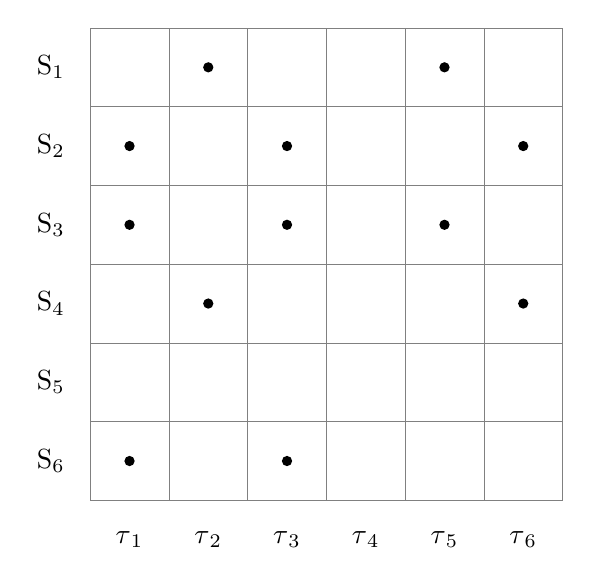
\begin{tikzpicture}
\node[draw=none] at (-.5,.5) {S\textsubscript{6}};
\node[draw=none] at (-.5,1.5) {S\textsubscript{5}};
\node[draw=none] at (-.5,2.5) {S\textsubscript{4}};
\node[draw=none] at (-.5,3.5) {S\textsubscript{3}};
\node[draw=none] at (-.5,4.5) {S\textsubscript{2}};
\node[draw=none] at (-.5,5.5) {S\textsubscript{1}};

\node[draw=none] at (.5,-.5) {$\tau \textsubscript{1}$};
\node[draw=none] at (1.5,-.5) {$\tau \textsubscript{2}$};
\node[draw=none] at (2.5,-.5) {$\tau \textsubscript{3}$};
\node[draw=none] at (3.5,-.5) {$\tau \textsubscript{4}$};
\node[draw=none] at (4.5,-.5) {$\tau \textsubscript{5}$};
\node[draw=none] at (5.5,-.5) {$\tau \textsubscript{6}$};

\draw[black, thick, fill] (1.5,5.5) circle(.05cm);
\draw[black, thick, fill] (4.5,5.5) circle(.05cm);

\draw[black, thick, fill] (.5,4.5) circle(.05cm);
\draw[black, thick, fill] (2.5,4.5) circle(.05cm);
\draw[black, thick, fill] (5.5,4.5) circle(.05cm);

\draw[black, thick, fill] (.5,3.5) circle(.05cm);
\draw[black, thick, fill] (2.5,3.5) circle(.05cm);
\draw[black, thick, fill] (4.5,3.5) circle(.05cm);

\draw[black, thick, fill] (1.5,2.5) circle(.05cm);
\draw[black, thick, fill] (5.5,2.5) circle(.05cm);


\draw[black, thick, fill] (.5,.5) circle(.05cm);
\draw[black, thick, fill] (2.5,.5) circle(.05cm);


\draw[step=1cm,gray,very thin] (0,0) grid (6,6);
\end{tikzpicture}
\end{center}

If $Sq$ is a valid TAP, then it must be true that for some quantum $\tau\textsubscript{j}$, it must start at $\tau\textsubscript{j}$ in at least $\alpha$ sequences. Thus for each $\tau\textsubscript{j}$, we can simply count how many dots we encounter in that column(refer the figure above). If for some $\tau\textsubscript{j}$, the number of dots is more than $\alpha$, then $Sq$ is a valid TAP starting in quantum $j$. Else it is not a TAP and can be discarded. 

\end{itemize}

\end{document}
